\section{Results and Discussion}
\label{sec:fn_opt:results}

    This section elucidates the optimization outcomes for 20 classical functions, analyzed using three distinct selection 
    strategies: Random, Tournament, and Roulette. The following tables and figures provide an in-depth view of the time 
    efficiency and effectiveness of each phase in the evolutionary process, along with the resultant optimization 
    performance.

    \begin{figure}[ht!]
        \centering
        \begin{subfigure}{.45\textwidth}
            \centering  
            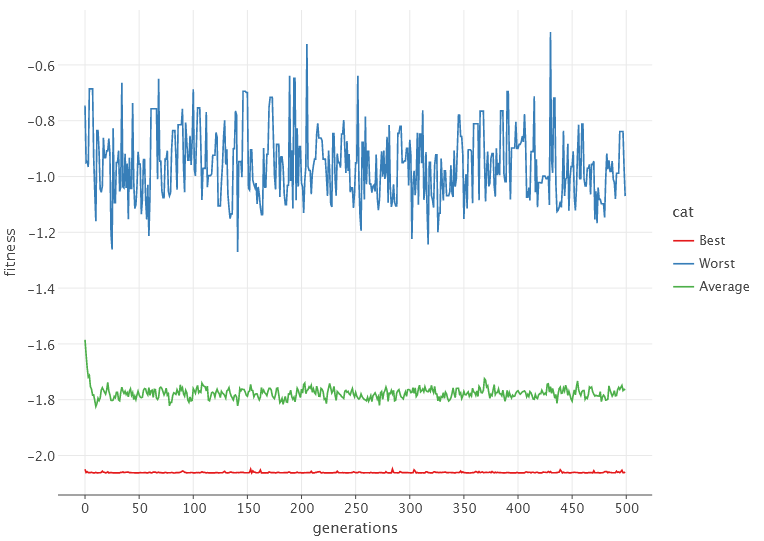
\includegraphics[width=\linewidth]{img/cross_in_tray_random.png}
            \caption{Random Selector}
        \end{subfigure}
        \begin{subfigure}{.45\textwidth}
            \centering
            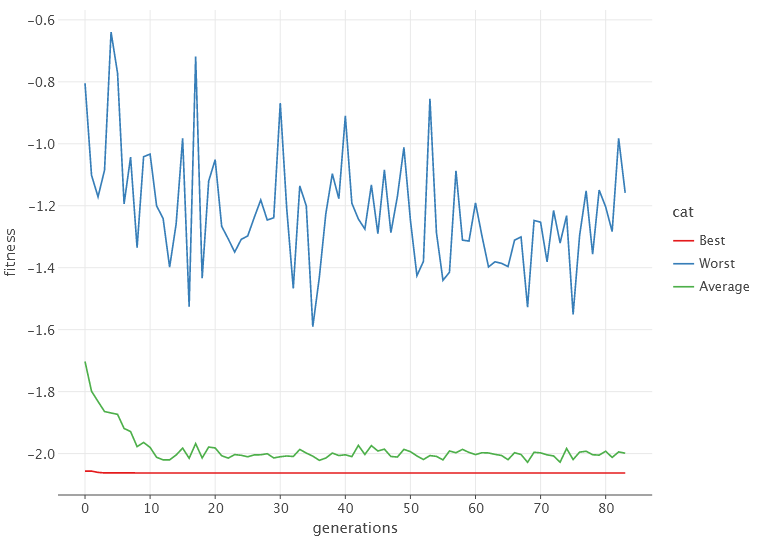
\includegraphics[width=\linewidth]{img/cross_in_tray_tournament.png}
            \caption{Tournament Selector}
        \end{subfigure}
        \begin{subfigure}{.45\textwidth}
            \centering
            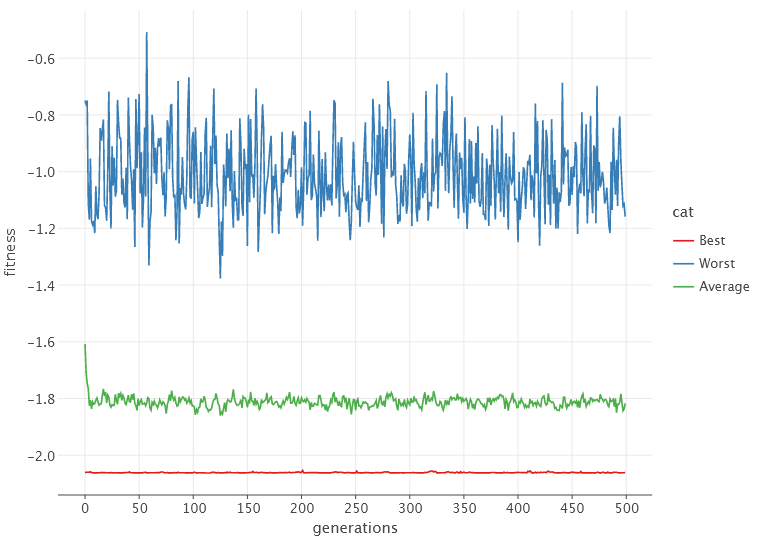
\includegraphics[width=\linewidth]{img/cross_in_tray_roulette.png}
            \caption{Roulette Selector}
        \end{subfigure}
        \caption{Fitness evolution for the Cross-in-tray function under different selection strategies.}
        \label{fig:fn_opt:results:cross_in_tray}
    \end{figure}

    The comparative analysis of the selectors, as depicted in \vref{fig:fn_opt:results:cross_in_tray}, highlights the 
    superior performance of the Tournament Selector over the Random and Roulette Selectors. Notably, the Random and 
    Roulette selectors exhibit comparable outcomes, which can be attributed to the inherent nature of the Roulette 
    Selector. This selector functions as a probabilistic version of the Random Selector, where the selection probability 
    is guided by individual fitness weights. As the evolutionary process progresses, the variance in these weights 
    diminishes, leading to Roulette Selector's behavior increasingly resembling that of the Random Selector.

    It is crucial to observe that while both Random and Roulette selectors occasionally approach or even achieve the
    global optimum, their inherent randomness impedes consistent maintenance of the optimum solution. Conversely, the 
    Tournament Selector, with its more deterministic and competitive selection mechanism, not only reaches but also 
    reliably sustains the optimal solutions once discovered. From this we can conclude that a stagnation termination
    criterion is not suitable for the Random and Roulette selectors, as they are not able to maintain the optimal 
    solution for a long enough period of time, instead a target fitness criterion may be more appropriate.

    Now we will present the results of the optimization process for each selector for each function.
    Each experiment was run 4 times, dropping the first iteration to avoid JVM warmup effects. The results presented are
    the average of the remaining 3 iterations.

    \newpage
    \begin{center}
        \subsection{Random Selector}
            \subimport{results/}{Random.tex}
        \subsection{Tournament Selector}
            \subimport{results/}{Tournament.tex}
        \subsection{Roulette Selector}
            \subimport{results/}{Roulette.tex}
    \end{center}

    A primary observation from the analysis is the minimal standard deviation in selection times across all selectors, 
    suggesting remarkable stability and consistency in the selection phase. Notably, the Random Selector exhibits the 
    lowest average selection time, attributed to its lack of computational requirements for individual selection. In 
    contrast, both the Tournament and Roulette selectors show comparable average selection times, with the Roulette 
    selector marginally slower. This slight increase in time for the Roulette selector stems from its necessity to 
    calculate fitness weights for each individual - a more computationally demanding task than the Tournament selector's 
    simple fitness comparison.

    When examining average evolution times, we find that they are relatively similar across all selectors, approximately 
    in the order of \(10^{-1}\) seconds. The Tournament selector, however, demonstrates a marginal speed advantage. This 
    efficiency is linked to its ability to avoid iterating through all generations to find an adequate solution, as it 
    effectively maintains the optimal solution once discovered. The Roulette selector, in comparison, is slightly slower 
    than the Random selector due to the additional computational load of fitness weight calculations.

    Focusing on the evolution outcomes, a distinct advantage of the Tournament selector emerges. It uniquely halts the 
    evolutionary process before reaching the maximum generation limit, achieving 50 steady generations earlier. This 
    efficiency is rooted in its capability to sustain an optimal solution once it is identified, unlike the other 
    selectors.

    Further analysis reveals that the Tournament selector consistently yields the lowest average error, indicating its 
    superiority in finding the most optimal solutions. The Roulette and Random selectors exhibit similar average errors, 
    with the Roulette selector slightly outperforming the Random one. This observation is reinforced by the lower 
    standard deviation in error for the Roulette selector, implying greater consistency in its results.

    Notable exceptions to the Tournament selector's low error performance are observed with the Rastrigin, Egg Holder, 
    and Schaffer functions. These functions are characterized by multiple, evenly distributed local optima, posing a 
    significant challenge for the algorithm to escape once convergence is achieved. Consequently, this leads to the 
    Tournament selector's inability to locate the global optimum in these cases. In contrast, functions like Booth, with 
    a single global optimum and a limited set of local optima, present a less complex landscape, enabling easier escape 
    and convergence to the global optimum.
